\documentclass[ignorenonframetext,]{beamer}
\setbeamertemplate{caption}[numbered]
\setbeamertemplate{caption label separator}{: }
\setbeamercolor{caption name}{fg=normal text.fg}
\beamertemplatenavigationsymbolsempty
\usepackage{lmodern}
\usepackage{amssymb,amsmath}
\usepackage{ifxetex,ifluatex}
\usepackage{fixltx2e} % provides \textsubscript
\ifnum 0\ifxetex 1\fi\ifluatex 1\fi=0 % if pdftex
  \usepackage[T1]{fontenc}
  \usepackage[utf8]{inputenc}
\else % if luatex or xelatex
  \ifxetex
    \usepackage{mathspec}
  \else
    \usepackage{fontspec}
  \fi
  \defaultfontfeatures{Ligatures=TeX,Scale=MatchLowercase}
\fi
% use upquote if available, for straight quotes in verbatim environments
\IfFileExists{upquote.sty}{\usepackage{upquote}}{}
% use microtype if available
\IfFileExists{microtype.sty}{%
\usepackage{microtype}
\UseMicrotypeSet[protrusion]{basicmath} % disable protrusion for tt fonts
}{}
\newif\ifbibliography
\hypersetup{
            pdftitle={Introduction to R markdown},
            pdfauthor={DSP作者群},
            pdfborder={0 0 0},
            breaklinks=true}
\urlstyle{same}  % don't use monospace font for urls
\usepackage{color}
\usepackage{fancyvrb}
\newcommand{\VerbBar}{|}
\newcommand{\VERB}{\Verb[commandchars=\\\{\}]}
\DefineVerbatimEnvironment{Highlighting}{Verbatim}{commandchars=\\\{\}}
% Add ',fontsize=\small' for more characters per line
\usepackage{framed}
\definecolor{shadecolor}{RGB}{248,248,248}
\newenvironment{Shaded}{\begin{snugshade}}{\end{snugshade}}
\newcommand{\KeywordTok}[1]{\textcolor[rgb]{0.13,0.29,0.53}{\textbf{#1}}}
\newcommand{\DataTypeTok}[1]{\textcolor[rgb]{0.13,0.29,0.53}{#1}}
\newcommand{\DecValTok}[1]{\textcolor[rgb]{0.00,0.00,0.81}{#1}}
\newcommand{\BaseNTok}[1]{\textcolor[rgb]{0.00,0.00,0.81}{#1}}
\newcommand{\FloatTok}[1]{\textcolor[rgb]{0.00,0.00,0.81}{#1}}
\newcommand{\ConstantTok}[1]{\textcolor[rgb]{0.00,0.00,0.00}{#1}}
\newcommand{\CharTok}[1]{\textcolor[rgb]{0.31,0.60,0.02}{#1}}
\newcommand{\SpecialCharTok}[1]{\textcolor[rgb]{0.00,0.00,0.00}{#1}}
\newcommand{\StringTok}[1]{\textcolor[rgb]{0.31,0.60,0.02}{#1}}
\newcommand{\VerbatimStringTok}[1]{\textcolor[rgb]{0.31,0.60,0.02}{#1}}
\newcommand{\SpecialStringTok}[1]{\textcolor[rgb]{0.31,0.60,0.02}{#1}}
\newcommand{\ImportTok}[1]{#1}
\newcommand{\CommentTok}[1]{\textcolor[rgb]{0.56,0.35,0.01}{\textit{#1}}}
\newcommand{\DocumentationTok}[1]{\textcolor[rgb]{0.56,0.35,0.01}{\textbf{\textit{#1}}}}
\newcommand{\AnnotationTok}[1]{\textcolor[rgb]{0.56,0.35,0.01}{\textbf{\textit{#1}}}}
\newcommand{\CommentVarTok}[1]{\textcolor[rgb]{0.56,0.35,0.01}{\textbf{\textit{#1}}}}
\newcommand{\OtherTok}[1]{\textcolor[rgb]{0.56,0.35,0.01}{#1}}
\newcommand{\FunctionTok}[1]{\textcolor[rgb]{0.00,0.00,0.00}{#1}}
\newcommand{\VariableTok}[1]{\textcolor[rgb]{0.00,0.00,0.00}{#1}}
\newcommand{\ControlFlowTok}[1]{\textcolor[rgb]{0.13,0.29,0.53}{\textbf{#1}}}
\newcommand{\OperatorTok}[1]{\textcolor[rgb]{0.81,0.36,0.00}{\textbf{#1}}}
\newcommand{\BuiltInTok}[1]{#1}
\newcommand{\ExtensionTok}[1]{#1}
\newcommand{\PreprocessorTok}[1]{\textcolor[rgb]{0.56,0.35,0.01}{\textit{#1}}}
\newcommand{\AttributeTok}[1]{\textcolor[rgb]{0.77,0.63,0.00}{#1}}
\newcommand{\RegionMarkerTok}[1]{#1}
\newcommand{\InformationTok}[1]{\textcolor[rgb]{0.56,0.35,0.01}{\textbf{\textit{#1}}}}
\newcommand{\WarningTok}[1]{\textcolor[rgb]{0.56,0.35,0.01}{\textbf{\textit{#1}}}}
\newcommand{\AlertTok}[1]{\textcolor[rgb]{0.94,0.16,0.16}{#1}}
\newcommand{\ErrorTok}[1]{\textcolor[rgb]{0.64,0.00,0.00}{\textbf{#1}}}
\newcommand{\NormalTok}[1]{#1}
\usepackage{longtable,booktabs}
\usepackage{caption}
% These lines are needed to make table captions work with longtable:
\makeatletter
\def\fnum@table{\tablename~\thetable}
\makeatother
\usepackage{graphicx,grffile}
\makeatletter
\def\maxwidth{\ifdim\Gin@nat@width>\linewidth\linewidth\else\Gin@nat@width\fi}
\def\maxheight{\ifdim\Gin@nat@height>\textheight0.8\textheight\else\Gin@nat@height\fi}
\makeatother
% Scale images if necessary, so that they will not overflow the page
% margins by default, and it is still possible to overwrite the defaults
% using explicit options in \includegraphics[width, height, ...]{}
\setkeys{Gin}{width=\maxwidth,height=\maxheight,keepaspectratio}

% Prevent slide breaks in the middle of a paragraph:
\widowpenalties 1 10000
\raggedbottom

\AtBeginPart{
  \let\insertpartnumber\relax
  \let\partname\relax
  \frame{\partpage}
}
\AtBeginSection{
  \ifbibliography
  \else
    \let\insertsectionnumber\relax
    \let\sectionname\relax
    \frame{\sectionpage}
  \fi
}
\AtBeginSubsection{
  \let\insertsubsectionnumber\relax
  \let\subsectionname\relax
  \frame{\subsectionpage}
}

\setlength{\parindent}{0pt}
\setlength{\parskip}{6pt plus 2pt minus 1pt}
\setlength{\emergencystretch}{3em}  % prevent overfull lines
\providecommand{\tightlist}{%
  \setlength{\itemsep}{0pt}\setlength{\parskip}{0pt}}
\setcounter{secnumdepth}{0}

\title{Introduction to R markdown}
\subtitle{Dynamic documents for R}
\author{DSP作者群}
\date{2019-05}

\begin{document}
\frame{\titlepage}

\begin{frame}{What does data analyst do?}

\\
\url{http://goo.gl/52THNf}

\end{frame}

\begin{frame}{What does data analyst actually do}

\\
\url{https://www.coursera.org/course/repdata}

\end{frame}

\begin{frame}{Why you need R Markdown?}

\begin{itemize}
\tightlist
\item
  \textbf{資料分析}做不完\\
\item
  \textbf{說明文件}沒空寫\\
\item
  \textbf{教授}要求換方法\\
\item
  \textbf{老闆}說要改流程\\
\item
  \textbf{客戶}要我做做看\\
\item
  年度報告要總結
\end{itemize}

\end{frame}

\begin{frame}{Why you need R Markdown}

\\
\url{http://goo.gl/YiJrlI}

\end{frame}

\begin{frame}{What is R Markdown?}

A convenient tool to generate reproducible documents.

\begin{itemize}
\tightlist
\item
  \href{http://daringfireball.net/projects/markdown/basics}{Markdown}

  \begin{itemize}
  \tightlist
  \item
    Lightweight markup language
  \item
    Remove HTML tag for higher readibility.
  \item
    Inline HTML is avaliable.
  \end{itemize}
\item
  R markdown

  \begin{itemize}
  \tightlist
  \item
    Markdown + embedded R code chunks
  \item
    (.Rmd) -\textgreater{} (.md) -\textgreater{} (.html, .docx, .pdf)
  \end{itemize}
\end{itemize}

\end{frame}

\begin{frame}[fragile]{Why R Markdown}

\begin{itemize}
\tightlist
\item
  製作reproducible的報告、投影片: \texttt{document} 、 \texttt{slides}
\item
  想寫數學式子好展現自己的專業 \(e=mc^2\): \texttt{mathjax}
\item
  只有一份source code,不需要額外複製圖片到報告中: \texttt{.rmd}
\item
  需求更改時,可以動態改變報告內容: \texttt{integrated\ shiny}
\item
  增加資料分析演算法的可讀性: \texttt{code\ and\ text}
\item
  HTML的報告和投影片的格式方便瀏覽: \texttt{html}
\item
  IDE? RStudio提供支援: \texttt{Knit\ Button}
\end{itemize}

\end{frame}

\begin{frame}[fragile]{Installation}

\begin{itemize}
\tightlist
\item
  最新版的RStudio已經包含R Markdown功能\\
\item
  你也可以透過以下指令安裝R Markdown套件:
\end{itemize}

\begin{Shaded}
\begin{Highlighting}[]
\KeywordTok{install.packages}\NormalTok{(}\StringTok{"rmarkdown"}\NormalTok{)}
\end{Highlighting}
\end{Shaded}

\end{frame}

\section{R Markdown 快速導覽}\label{r-markdown-}

\begin{frame}{Overview}

\end{frame}

\begin{frame}{Markdown}

\end{frame}

\begin{frame}{R Code Chunks}

\end{frame}

\begin{frame}[fragile]{Inline R Code}

\begin{itemize}
\tightlist
\item
  利用 `r` 在markdown中插入R程式
\end{itemize}

\begin{verbatim}
- 這是DSP推出的第 `r 3+1`門課程  
\end{verbatim}

\begin{itemize}
\tightlist
\item
  這是DSP推出的第 4門課程
\end{itemize}

\begin{verbatim}
- 鳶尾花資料集(iris dataset)有 `r levels(iris$Species)` 等種類,
  總共有 `r length(levels(iris$Species))` 種
\end{verbatim}

\begin{itemize}
\tightlist
\item
  鳶尾花資料集(iris dataset)有 setosa, versicolor, virginica 等種類,\\
  總共有 3 種
\end{itemize}

\end{frame}

\begin{frame}[fragile]{Inline R Equations}

\begin{itemize}
\tightlist
\item
  插入 LaTeX 公式的方法:\\
\item
  行內\texttt{\$\ equation\ \$}\\
\item
  段落 \texttt{\$\$\ equation\ \$\$}
\end{itemize}

\begin{verbatim}
熵指標的公式為 $-\sum{p_i \log{p_i}}$ ,表示系統的亂度  
\end{verbatim}

熵指標的公式為 \(-\sum{p_i \log{p_i}}\) ,表示系統的亂度

\begin{verbatim}
請計算高斯分佈 $$f(x;\mu,\sigma^2) = \frac{1}{\sigma\sqrt{2\pi}} 
e^{ -\frac{1}{2}\left(\frac{x-\mu}{\sigma}\right)^2 }$$  
\end{verbatim}

請計算高斯分佈
\[f(x;\mu,\sigma^2) = \frac{1}{\sigma\sqrt{2\pi}} e^{ -\frac{1}{2}\left(\frac{x-\mu}{\sigma}\right)^2 }\]

\end{frame}

\begin{frame}[fragile]{Rendering Output}

\begin{itemize}
\tightlist
\item
  RStudio: ``Knit'' command:

  \begin{itemize}
  \tightlist
  \item
    (Win:Ctrl+Shift+K / OSX:Command+Shirt+K)\\
  \end{itemize}
\item
  Command line: rmarkdown::render function
\end{itemize}

\begin{Shaded}
\begin{Highlighting}[]
\NormalTok{rmarkdown}\OperatorTok{::}\KeywordTok{render}\NormalTok{(}\StringTok{"input.Rmd"}\NormalTok{)}
\end{Highlighting}
\end{Shaded}

\end{frame}

\section{Markdown Basics}\label{markdown-basics}

\begin{frame}[fragile]{Markdown Quick Reference}

在RStudio中,在UI界面中點選\texttt{help\ (?)}可以查閱Markdown語法\\

\end{frame}

\section{R Code Chunks}\label{r-code-chunks-1}

\begin{frame}[fragile]{Overview}

R code will be evaluated and printed

\begin{Shaded}
\begin{Highlighting}[]
\KeywordTok{summary}\NormalTok{(cars}\OperatorTok{$}\NormalTok{dist)}
\end{Highlighting}
\end{Shaded}

\begin{verbatim}
   Min. 1st Qu.  Median    Mean 3rd Qu.    Max. 
      2      26      36      43      56     120 
\end{verbatim}

\end{frame}

\begin{frame}[fragile]{Overview (cont.)}

draw graphics

\begin{Shaded}
\begin{Highlighting}[]
\KeywordTok{plot}\NormalTok{(women)  }
\end{Highlighting}
\end{Shaded}

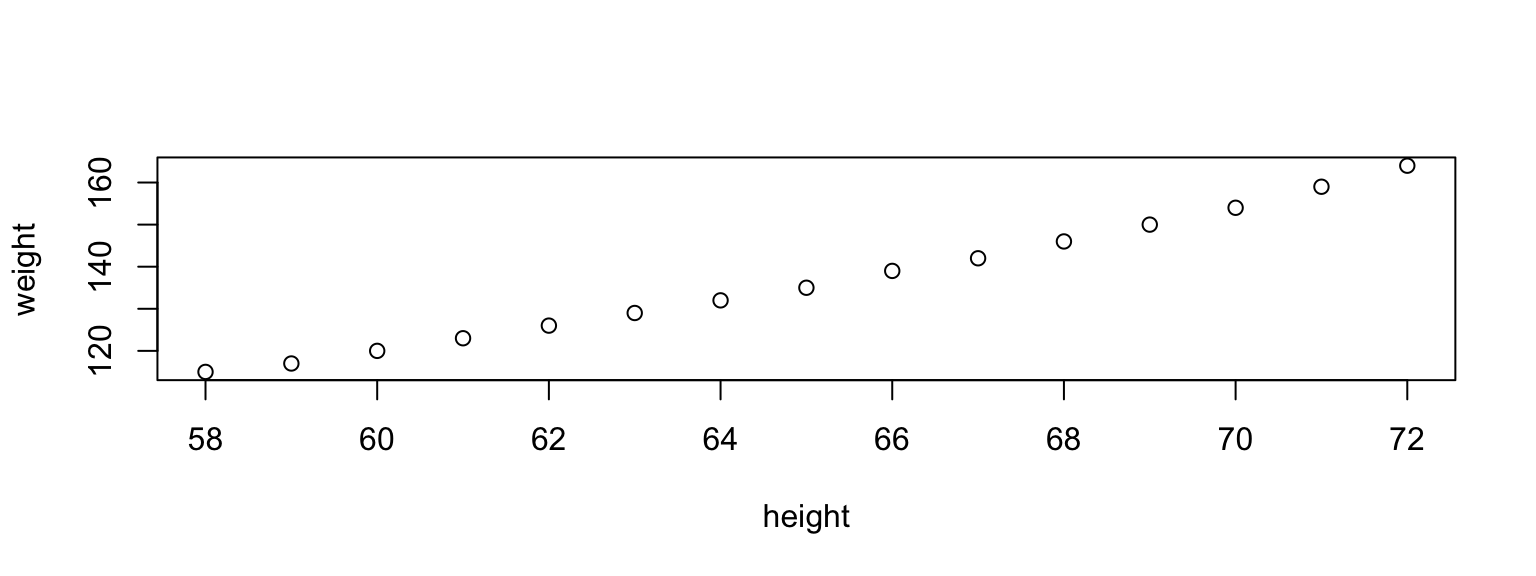
\includegraphics{R_markdown_files/figure-beamer/plot1-1.pdf}

\end{frame}

\begin{frame}{Named R code chunk.}

\begin{itemize}
\tightlist
\item
  Easy Navigation in RStudio
\end{itemize}

\end{frame}

\begin{frame}[fragile]{Basic Chunk Options}

\begin{itemize}
\tightlist
\item
  \texttt{echo}(TRUE): whether to include R source code in the output
  file\\
\item
  \texttt{eval}(TRUE): whether to evaluate the code chunk\\
\item
  \texttt{message}(TRUE): whether to preserve messages emitted by
  message()\\
\item
  \texttt{results}(`hide',`asis'): hide output ; asis treats the output
  of your R code as literal Markdown (when using like kable function)\\
\item
  \texttt{include}(TRUE): whether to be written into the output
  document, but the code is still evaluated and plot files are
  generated\\
\item
  \texttt{warning}(TRUE): whether to preserve warnings in the output
\item
  \texttt{comment}(``\#\#''): set to comment notation
\end{itemize}

\end{frame}

\begin{frame}[fragile]{Basic Chunk Options (cont.)}

Set global chunk options at code chunks header:

\begin{Shaded}
\begin{Highlighting}[]
\NormalTok{knitr}\OperatorTok{::}\NormalTok{opts_chunk}\OperatorTok{$}\KeywordTok{set}\NormalTok{(}\DataTypeTok{echo=}\OtherTok{FALSE}\NormalTok{, }\DataTypeTok{results=}\StringTok{'hide'}\NormalTok{)}
\end{Highlighting}
\end{Shaded}

\end{frame}

\begin{frame}{Exercise:}

利用R Markdown
製作《一周天氣預報》書面報告。\href{https://dspim.github.io/A1-basic-data-analysis/RMD-example/RmdExAns.html}{範例}\\
*
\href{http://www.cwb.gov.tw/V7/forecast/taiwan/Taipei_City.htm}{原始出處}\\
*
\href{https://github.com/dspim/a1-basic-data-analysis-course/blob/master/RmdExQue.Rmd}{參考範本}\\
*
\href{https://github.com/dspim/a1-basic-data-analysis-course/blob/master/data/weather-utf8.csv}{範例資料}

\end{frame}

\begin{frame}{Exercise: Original:}

\end{frame}

\begin{frame}{Exercise: After:}

\end{frame}

\begin{frame}[fragile]{Exercise Q1}

利用R Markdown 製作《一周天氣預報》書面報告。 -
計算01/28日當日的最高溫與最低溫度

\begin{Shaded}
\begin{Highlighting}[]
\CommentTok{# Hint:}
\CommentTok{# 1. 下載weather-utf8.csv到自己的電腦上}
\CommentTok{# 2. 在R chunk中,利用read.csv()讀取檔案進行分析}
  \CommentTok{#  Windows: read.csv(,fileEncoding="UTF-8")}
\CommentTok{# 3. 找出01/28當日最高溫 max()}
\CommentTok{# 4. 找出01/28當日最低溫 min()}
\CommentTok{# 5. use inline R chunk `r max(...)` }
\end{Highlighting}
\end{Shaded}

\end{frame}

\begin{frame}[fragile]{Exercise A1}

利用R Markdown 製作《一周天氣預報》書面報告。 -
計算01/28日當日的最高溫與最低溫度

\begin{Shaded}
\begin{Highlighting}[]
\CommentTok{# Hint for Linux & Mac:}
\NormalTok{dat <-}\StringTok{ }\KeywordTok{read.csv}\NormalTok{(}\StringTok{"data/weather-utf8.csv"}\NormalTok{) }
\KeywordTok{max}\NormalTok{(dat[}\DecValTok{1}\OperatorTok{:}\DecValTok{2}\NormalTok{, }\DecValTok{4}\OperatorTok{:}\DecValTok{5}\NormalTok{])}
\KeywordTok{min}\NormalTok{(dat[}\DecValTok{1}\OperatorTok{:}\DecValTok{2}\NormalTok{, }\DecValTok{4}\OperatorTok{:}\DecValTok{5}\NormalTok{])}
\CommentTok{# 預測高溫約`r max(dat[1:2,4:5])`度,低溫約`r min(dat[1:2,4:5])`度}
\end{Highlighting}
\end{Shaded}

\begin{Shaded}
\begin{Highlighting}[]
\CommentTok{# Hint for Windows:}
\NormalTok{dat <-}\StringTok{ }\KeywordTok{read.csv}\NormalTok{(}\StringTok{"data/weather-utf8.csv"}\NormalTok{, }\DataTypeTok{fileEncoding=}\StringTok{"UTF-8"}\NormalTok{) }
\KeywordTok{max}\NormalTok{(dat[}\DecValTok{1}\OperatorTok{:}\DecValTok{2}\NormalTok{, }\DecValTok{4}\OperatorTok{:}\DecValTok{5}\NormalTok{])}
\KeywordTok{min}\NormalTok{(dat[}\DecValTok{1}\OperatorTok{:}\DecValTok{2}\NormalTok{, }\DecValTok{4}\OperatorTok{:}\DecValTok{5}\NormalTok{])}
\CommentTok{# 預測高溫約`r max(dat[1:2,4:5])`度,低溫約`r min(dat[1:2,4:5])`度}
\end{Highlighting}
\end{Shaded}

\end{frame}

\begin{frame}[fragile]{Table Output}

\begin{itemize}
\tightlist
\item
  Print data directly:
\end{itemize}

\begin{Shaded}
\begin{Highlighting}[]
\KeywordTok{print}\NormalTok{(}\KeywordTok{head}\NormalTok{(women))}
\end{Highlighting}
\end{Shaded}

\begin{verbatim}
  height weight
1     58    115
2     59    117
3     60    120
4     61    123
5     62    126
6     63    129
\end{verbatim}

\end{frame}

\begin{frame}[fragile]{Table Output (cont.)}

\begin{itemize}
\tightlist
\item
  Using \texttt{knitr::kable} :

  \begin{itemize}
  \tightlist
  \item
    Set \texttt{results=\textquotesingle{}asis\textquotesingle{}} to
    write raw results from R into the output document\\
  \end{itemize}
\end{itemize}

\begin{longtable}[]{@{}rr@{}}
\toprule
height & weight\tabularnewline
\midrule
\endhead
58 & 115\tabularnewline
59 & 117\tabularnewline
60 & 120\tabularnewline
61 & 123\tabularnewline
62 & 126\tabularnewline
63 & 129\tabularnewline
\bottomrule
\end{longtable}

\end{frame}

\begin{frame}[fragile]{Exercise Q2}

利用R Markdown 製作《一周天氣預報》書面報告。 - 製作未來七天天氣預報表

\begin{Shaded}
\begin{Highlighting}[]
\CommentTok{# Hint:}
\CommentTok{# 你可能需要dplyr套件}
\CommentTok{# 可以先用filter把白天、晚上分開處理}
\CommentTok{# 利用 paste(低溫,高溫,sep="-") 來製作溫度區間, i.e. 16-17}
\CommentTok{# 利用colnames, rownames來對整理好的資料表的行與列命名}
\end{Highlighting}
\end{Shaded}

\end{frame}

\begin{frame}[fragile]{Exercise A2}

利用R Markdown 製作《一周天氣預報》書面報告。 - 製作未來七天天氣預報表

\begin{Shaded}
\begin{Highlighting}[]
\KeywordTok{library}\NormalTok{(dplyr)}
\NormalTok{day1 <-}\StringTok{ }\KeywordTok{filter}\NormalTok{(dat, 早晚}\OperatorTok{==}\StringTok{"白天"}\NormalTok{)}
\NormalTok{day2 <-}\StringTok{ }\KeywordTok{mutate}\NormalTok{(day1, 溫度=}\KeywordTok{paste}\NormalTok{(高溫,低溫,}\DataTypeTok{sep=}\StringTok{"-"}\NormalTok{))}
\NormalTok{day3 <-}\StringTok{ }\KeywordTok{select}\NormalTok{(day2, 天氣, 溫度)}

\NormalTok{night1 <-}\StringTok{ }\KeywordTok{filter}\NormalTok{(dat, 早晚}\OperatorTok{==}\StringTok{"晚上"}\NormalTok{)}
\NormalTok{night2 <-}\StringTok{ }\KeywordTok{mutate}\NormalTok{(night1, 溫度=}\KeywordTok{paste}\NormalTok{(高溫,低溫,}\DataTypeTok{sep=}\StringTok{"-"}\NormalTok{))}
\NormalTok{night3 <-}\StringTok{ }\KeywordTok{select}\NormalTok{(night2, 天氣, 溫度)}

\NormalTok{out <-}\StringTok{ }\KeywordTok{data.frame}\NormalTok{(}\KeywordTok{t}\NormalTok{(}\KeywordTok{bind_cols}\NormalTok{(day3, night3)))}
\KeywordTok{colnames}\NormalTok{(out) <-}\StringTok{ }\NormalTok{day1}\OperatorTok{$}\NormalTok{日期}
\KeywordTok{rownames}\NormalTok{(out) <-}\StringTok{ }\KeywordTok{c}\NormalTok{(}\StringTok{"白天天氣"}\NormalTok{,}\StringTok{"白天溫度"}\NormalTok{,}\StringTok{"晚上天氣"}\NormalTok{,}\StringTok{"晚上溫度"}\NormalTok{)}
\end{Highlighting}
\end{Shaded}

\end{frame}

\begin{frame}{Exercise A2 (conti.)}

利用R Markdown 製作《一周天氣預報》書面報告。 - 製作未來七天天氣預報表

\end{frame}

\begin{frame}[fragile]{Exercise Q3}

利用R Markdown 製作《一周天氣預報》書面報告。 - 製作未來七天天氣預報圖

\begin{Shaded}
\begin{Highlighting}[]
\CommentTok{# Hint:}
\CommentTok{# 你可能需要ggplot2套件}
\CommentTok{# Mac顯示中文需設置字型}
  \CommentTok{# http://equation85.github.io/blog/graph-font-of-r-in-mac-os-x/}
  \CommentTok{# par(family='STHeiti')}
\end{Highlighting}
\end{Shaded}

\end{frame}

\begin{frame}[fragile]{Exercise A3}

利用R Markdown 製作《一周天氣預報》書面報告。 - 製作未來七天天氣預報圖

\begin{Shaded}
\begin{Highlighting}[]
\KeywordTok{library}\NormalTok{(ggplot2);}\KeywordTok{library}\NormalTok{(reshape2)}
\NormalTok{dat1 <-}\StringTok{ }\KeywordTok{mutate}\NormalTok{(dat, 時間=}\KeywordTok{paste}\NormalTok{(日期,早晚,}\DataTypeTok{sep=}\StringTok{"}\CharTok{\textbackslash{}n}\StringTok{"}\NormalTok{))}
\NormalTok{dat2 <-}\StringTok{ }\KeywordTok{select}\NormalTok{(dat1, 時間, 高溫, 低溫)}
\KeywordTok{colnames}\NormalTok{(dat2)[}\DecValTok{1}\NormalTok{] <-}\StringTok{ "時間"} \CommentTok{# for Windows user}
\NormalTok{dat3 <-}\StringTok{ }\KeywordTok{melt}\NormalTok{(dat2)}
\NormalTok{g <-}\StringTok{ }\KeywordTok{ggplot}\NormalTok{(dat3, }\KeywordTok{aes}\NormalTok{(}\DataTypeTok{x=}\NormalTok{時間, }\DataTypeTok{y=}\NormalTok{value, }\DataTypeTok{group=}\NormalTok{variable, }\DataTypeTok{colour=}\NormalTok{variable)) }\OperatorTok{+}\StringTok{ }
\StringTok{  }\KeywordTok{geom_line}\NormalTok{() }\OperatorTok{+}\StringTok{ }
\StringTok{  }\KeywordTok{labs}\NormalTok{(}\DataTypeTok{x=}\StringTok{"時間"}\NormalTok{, }\DataTypeTok{y=}\StringTok{"溫度"}\NormalTok{) }
\end{Highlighting}
\end{Shaded}

\begin{Shaded}
\begin{Highlighting}[]
\CommentTok{# 顯示中文字 Mac user only}
\NormalTok{g }\OperatorTok{+}\StringTok{ }\KeywordTok{theme_gray}\NormalTok{(}\DataTypeTok{base_family=}\StringTok{"STHeiti"}\NormalTok{) }
\end{Highlighting}
\end{Shaded}

\end{frame}

\begin{frame}{Exercise}

利用R Markdown 製作《一周天氣預報》書面報告。

\begin{itemize}
\tightlist
\item
  \href{http://www.cwb.gov.tw/V7/forecast/taiwan/Taipei_City.htm}{原始出處}
\item
  \href{https://github.com/dspim/a1-basic-data-analysis-course/blob/master/RmdExQue.Rmd}{參考範本}
\item
  \href{https://github.com/dspim/a1-basic-data-analysis-course/blob/master/data/weather-utf8.csv}{範例資料}
\item
  \href{https://github.com/dspim/a1-basic-data-analysis-course/blob/master/RmdExAns.Rmd}{參考解答}
\end{itemize}

\end{frame}

\section{Appendiex}\label{appendiex}

\begin{frame}{About Document Content}

You can add R Markdown and HTML in the YAML content.

\end{frame}

\begin{frame}{YAML metadata}

\\
Cover by Wush

\end{frame}

\begin{frame}[fragile]{Some Useful HTML}

\begin{itemize}
\item
  \href{http://www.w3schools.com/tags/tag_iframe.asp}{iframe}:
  displaying a web page within a web page

\begin{Shaded}
\begin{Highlighting}[]
\KeywordTok{<iframe}\OtherTok{ src=}\StringTok{"http://dsp.im/"}\OtherTok{ height=}\StringTok{600}\OtherTok{ width=}\StringTok{800}\KeywordTok{></iframe>}
\end{Highlighting}
\end{Shaded}
\item
  \href{http://www.w3schools.com/tags/tag_img.asp}{img}: inserting
  images into an HTML document. Much easier for adjusting width and
  height.

\begin{Shaded}
\begin{Highlighting}[]
\KeywordTok{<img}\OtherTok{ src=}\StringTok{"img/dsp-logo.png"}\OtherTok{ alt=}\StringTok{"logo"}\KeywordTok{>}
\end{Highlighting}
\end{Shaded}
\end{itemize}

\end{frame}

\begin{frame}{Interactive Documents}

It's possible to embed a Shiny application within a document.

\end{frame}

\begin{frame}[fragile]{Publish to the web}

Using R packages::slidify to publish your slides to the web

\begin{verbatim}
library(slidify)
publish_github("repo", username="user_name")
publish_rpubs("title","file_name.html")
publish_dropbox(dir_name)
publish_gist("title",file="file_name.html",publish=TRUE)
\end{verbatim}

\end{frame}

\begin{frame}{Publish to the web: Github}

\begin{enumerate}
\def\labelenumi{\arabic{enumi}.}
\tightlist
\item
  sign up or login in Github.com at browser
\item
  find button: New repository to add new one.
\item
  select a name for repository, then created.
\item
  the link of your new repository would be like:\\
  \href{https://github.com/your_name/repo_name.git}{https://github.com/``your\_name''/``repo\_name''.git}
\item
  find Settings in your profile at top-right corner
\item
  select SSH Keys and add SSH Key
\item
  upload your SSH key which created by your own PC/notebook.
\item
  at RStudio, using Rcommand:\\
  slidify::publish\_github(``repo\_name'', username=``your\_name'')
\item
  your new page will be ready in 5\textasciitilde{}10 min and link:\\
  \href{https://your_name.github.io/repo_name/index.html}{https://``your\_name''.github.io/``repo\_name''/index.html}
\end{enumerate}

\end{frame}

\begin{frame}{References}

\begin{itemize}
\tightlist
\item
  \href{http://mansunkuo.github.io/rmd_tutorial/}{An Introduction to R
  Markdown*} by Mansun Kuo @
  \href{http://taiwanrusergroup.github.io/DSC2014Tutorial/}{DSC2014}
\item
  \href{http://shiny.rstudio.com/articles/rm-cheatsheet.html}{R Markdown
  Cheat Sheet}
\item
  \href{http://rmarkdown.rstudio.com/}{R Markdown}
\item
  \href{http://yihui.name/knitr/}{knitr}
\item
  \href{https://support.rstudio.com/hc/en-us/categories/200035113-Documentation}{RStudio
  Documentation}
\item
  \href{https://www.coursera.org/course/repdata}{Reproducible Research}
\item
  \href{http://shiny.rstudio.com/articles/}{Shiny Articles}
\item
  \href{http://slidify.org/publish.html}{Publish to Github
  Pages/Dropbox/Rpubs}
\end{itemize}

\end{frame}

\begin{frame}{Wush 教學影片}

\href{https://www.youtube.com/watch?v=P97udK2ktuY}{Slidify簡介} by Wush
Wu\\
\url{https://www.youtube.com/watch?v=P97udK2ktuY}

\href{https://www.youtube.com/watch?v=OHKZLeKlUsM}{20121203 MLDM
Monday:markdown + knitr (Hangout 轉播)} by Wush Wu\\
\url{https://www.youtube.com/watch?v=OHKZLeKlUsM}

\end{frame}

\end{document}
